
%==========IMPLEMENTATION==========

\section{Implementation}
\begin{figure}[h!]
    \centering
    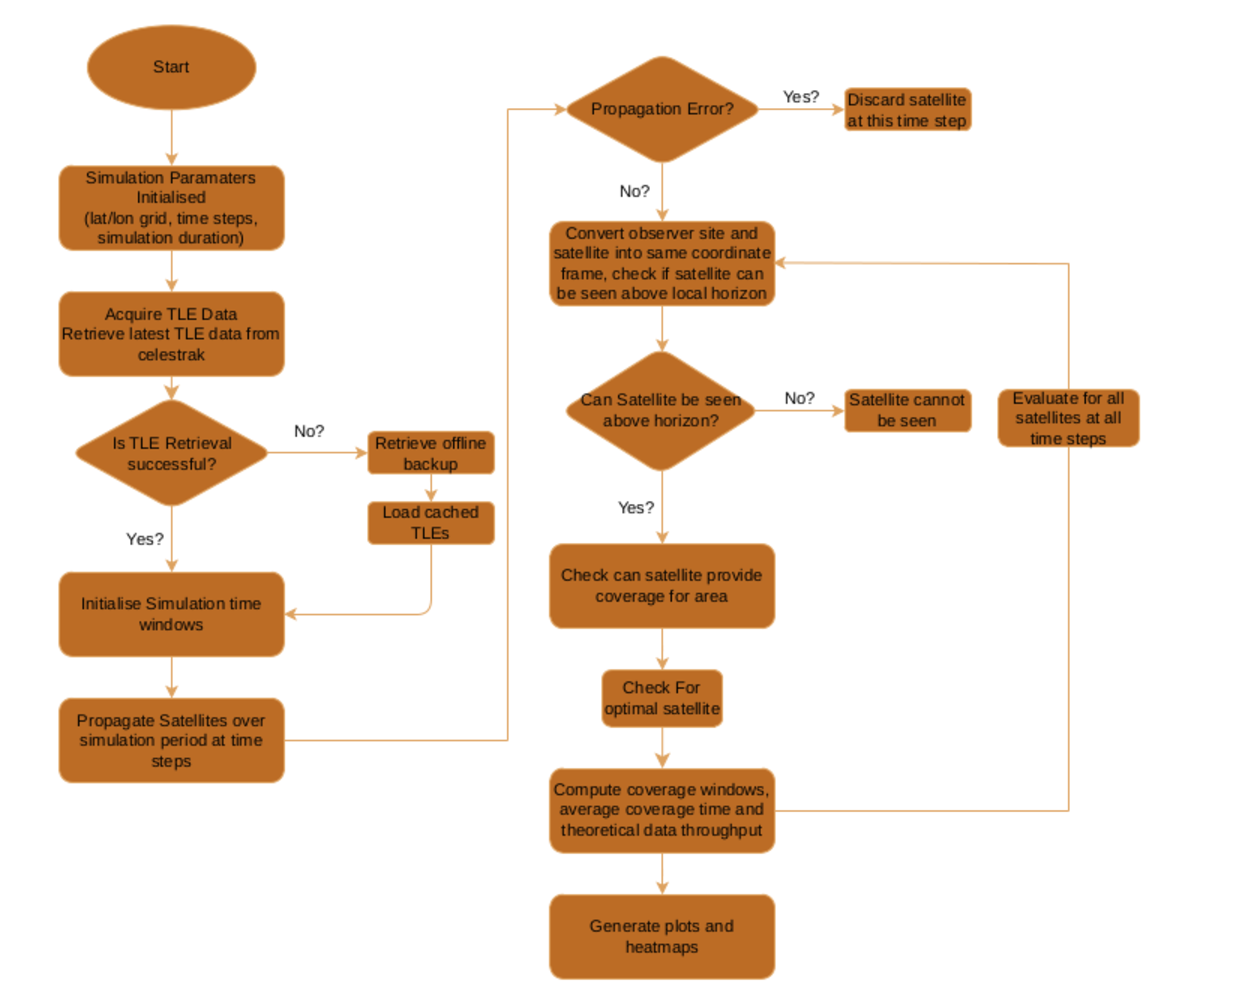
\includegraphics[width=0.8\linewidth]{figures/FYP_Overall_Logic.pdf}
    \caption{Implementation Logic}
    \label{fig:ImplementationLogic}
\end{figure}

The implementation of this project consists of a Python based system which retrieves live orbital data for LEO satellites using Celestrak and then propagates each orbit using the SGP4 model. Using these propagations, geometric visibility checks for specific locations are calculated.  The system is designed to support coverage and capacity calculations by determining which satellites are optimal for downlink access at a given period in time.  

\subsection{Data acquisition}
The first stage of implementation is acquiring up ot date orbital Parameters for the Starlink LEO constellation. TLE sets are retrieved from Celestrak. This data provides the perturbations required  to propagate the orbits using SGP4. The TLE data used in this system are taken directly from Celestrak \cite{celestrakTLE}. Downloading this data produces a text stream which has sets of three lines of text blocks, satellite name, followed by line 1 and line 2 of the TLE. The implementation of this system parses these entries for each satellite.  

Using live TLEs ensures that the system accurately represents the dynamic nature of large LEO constellations, which orbital parameters may change drastically and regularly due to any number of factors such as manual maneuvers. 

\subsection{Orbit propagation}
Once the TLEs have been retrieved and parsed in a suitable manner, each satellite's position and velocity are computed using the SGP4 algorithm. In this system each satellites state vector can be generated as seen in Listing \ref{code:sgp4}.

\begin{lstlisting}[language=Python, caption={SGP4 propagation example}, label={code:sgp4}]
satellite = Satrec.twoline2rv(line1, line2)
e, r, v = satellite.sgp4(jd, fr)
\end{lstlisting}


The outputs of the \ref{code:sgp4} are as follows:

\begin{itemize}
    \item \textbf{r}: The satellite position vector $\left(x, y, z\right)$ expressed in the True Equator Mean Equinox (TEME) reference frame.
    \item \textbf{v}: The satellite velocity vector in the TEME coordinate frame.
    \item \textbf{e}: An error flag returned by the propagator, where a value of zero indicates successful propagation and non-zero values correspond to specific SGP4 error conditions.
\end{itemize}

The Julian Date (jd, fr) is computed using the current UTC timestamp to ensure a precise propagation epoch. Any satellite with a non zero error flags are discarded to avoid propagating any invalid orbital data. 


\subsection{Coordinate Transformations}
Satellite positions produced by SGP4 are given in True Equator, Mean Equinox (TEME) format. TEME remains fixed to relative to the stars not to the Earth. It uses the Earths true equatorial plane at that moment in tim, but for the x-axis it uses the mean equinox which helps smooth out some of the short term wobbles in the Earths's rotation.  

As TEME does not rotate with the Earth, but ground locations given in latitude and longitude do rotate with the Earth, for visibility and elevation calculations, both the satellite and the observer location need to be in the same rotating frame. For this reason TEME must be converted to Earth Centered Earth Fixed (ECEF) coordinate system \cite{inproceedings}. 
 
\subsubsection{TEME to ECEF}
\endL
The conversion for TEME to ECEF is as follows \ldots

\begin{equation}
    \mathbf{r}_{\text{ECEF}} = R_{3}\!\left(\theta_{\text{GMST}}\right)\,\mathbf{r}_{\text{TEME}},
\end{equation}

\noindent\textbf{Where:}
\begin{itemize}
    \item $R_{3}(\theta)$ is a rotation matrix describing a rotation about the Earth's $Z$--axis.
    \item $\theta_{\text{GMST}}$ is the Greenwich Mean Sidereal Time at the observation epoch.
\end{itemize}

This can be written explicitly as a rotation matrix as follows \ldots

\begin{equation}
R_{3}(\theta) = 
\begin{bmatrix}
\cos\theta & -\sin\theta & 0 \\
\sin\theta &  \cos\theta & 0 \\
0          &  0          & 1
\end{bmatrix}
\end{equation}

Meaning \ldots

\begin{equation}
\begin{bmatrix}
x_{\text{ECEF}} \\
y_{\text{ECEF}} \\
z_{\text{ECEF}}
\end{bmatrix}
=
\begin{bmatrix}
\cos\theta_{\text{GMST}} & -\sin\theta_{\text{GMST}} & 0 \\
\sin\theta_{\text{GMST}} &  \cos\theta_{\text{GMST}} & 0 \\
0                        &  0                        & 1
\end{bmatrix}
\begin{bmatrix}
x_{\text{TEME}} \\
y_{\text{TEME}} \\
z_{\text{TEME}}
\end{bmatrix}
\end{equation}


\subsubsection{Latitude Longitude to ECEF}

\endL
\newline
\noindent\textbf{Given:}
\begin{itemize}
    \item Latitude: $\phi$ \, (radians)
    \item Longitude: $\lambda$ \, (radians)
    \item Altitude: $h$ \, (meters above the WGS--84 reference ellipsoid)
\end{itemize}


\noindent\textbf{WGS--84 Ellipsoid Constants:}
\begin{itemize}
    \item $a = 6378137.0 \ \text{m}$ \quad (equatorial radius)
    \item $f = \dfrac{1}{298.257223563}$ \quad (flattening)
    \item $e^{2} = 2f - f^{2}$ \quad (first eccentricity squared)
\end{itemize}

The first step is to find the distance from Earth's center to the surface at a given latitude \ldots


\begin{equation}
N(\phi) = \frac{a}{\sqrt{1 - e^{2}\sin^{2}\phi}}.
\end{equation}


Knowing this means it is now possible to compute the ECEF coordinate.


\begin{align}
X &= \left( N(\phi) + h \right)\cos\phi\cos\lambda \\[6pt]
Y &= \left( N(\phi) + h \right)\cos\phi\sin\lambda \\[6pt]
Z &= \left( N(\phi)(1 - e^{2}) + h \right)\sin\phi
\end{align}


\subsection{Visibility Logic}
Once both the ground observer and the satellites propagated position are represented in ECEF the first filter check for visibility can be applied. This is based on computing the satellite's elevation angle relative to the observers horizon. 

Given the satellite position,

\begin{equation}
     r_{\text{satellite}}^{\text{ECEF}} = (s_x, s_y, s_z),
\end{equation}



and the observer position, 


\begin{equation}
     r_{\text{observer}}^{\text{ECEF}} = (g_x, g_y, g_z),
\end{equation}

the line of sight vector (LOS) can be represented as,



\begin{equation}
     d = r_{\text{satellite}}^{\text{ECEF}} - r_{\text{observer}}^{\text{ECEF}}= (d_x, d_y, d_z),
\end{equation}

Using the observer latitude and longitude, the LOS can be converted into local horizon coordinates. This can be done following (\ref{eq:enu}) \cite{Navipedia_ECEF_ENU} 

\begin{equation} \label{eq:enu}
\begin{aligned}
e &= -\sin\lambda \, d_x + \cos\lambda \, d_y, \\
n &= -\cos\lambda \sin\phi \, d_x - \sin\lambda \sin\phi \, d_y + \cos\phi \, d_z, \\
u &= \cos\lambda \cos\phi \, d_x + \sin\lambda \cos\phi \, d_y + \sin\phi \, d_z.
\end{aligned}
\end{equation}

Using this, the elevation angle can then be computed as the angle between the LOS vector and the local horizon \cite{Navipedia_ECEF_ENU}. 

\begin{equation}
    \theta_{\text{el}} = \arctan\left( \frac{u}{\sqrt{e^2 + n^2}} \right)
\end{equation}

Then, to filter out any satellites which are too close to the horizon or below the horizon, a mask angle of $10^{\circ}$ is applied. 


\begin{equation}
    \text{el} \geq \theta_{\text{mask}}, \qquad 
    \theta_{\text{mask}} = 10^\circ
\end{equation}


\subsection{Coverage Loop}

\subsection{TLE offline Fallback}


\subsection{Visualisations}